\documentclass[border=10pt]{standalone}

\usepackage{tikz}
\usepackage{tikzsymbols}
\usetikzlibrary{calc,patterns,shapes.geometric}

\def\centerarc[#1](#2)(#3:#4:#5){\draw[#1] ($(#2)+({#5*cos(#3)},{#5*sin(#3)})$) arc (#3:#4:#5);}

\begin{document}
	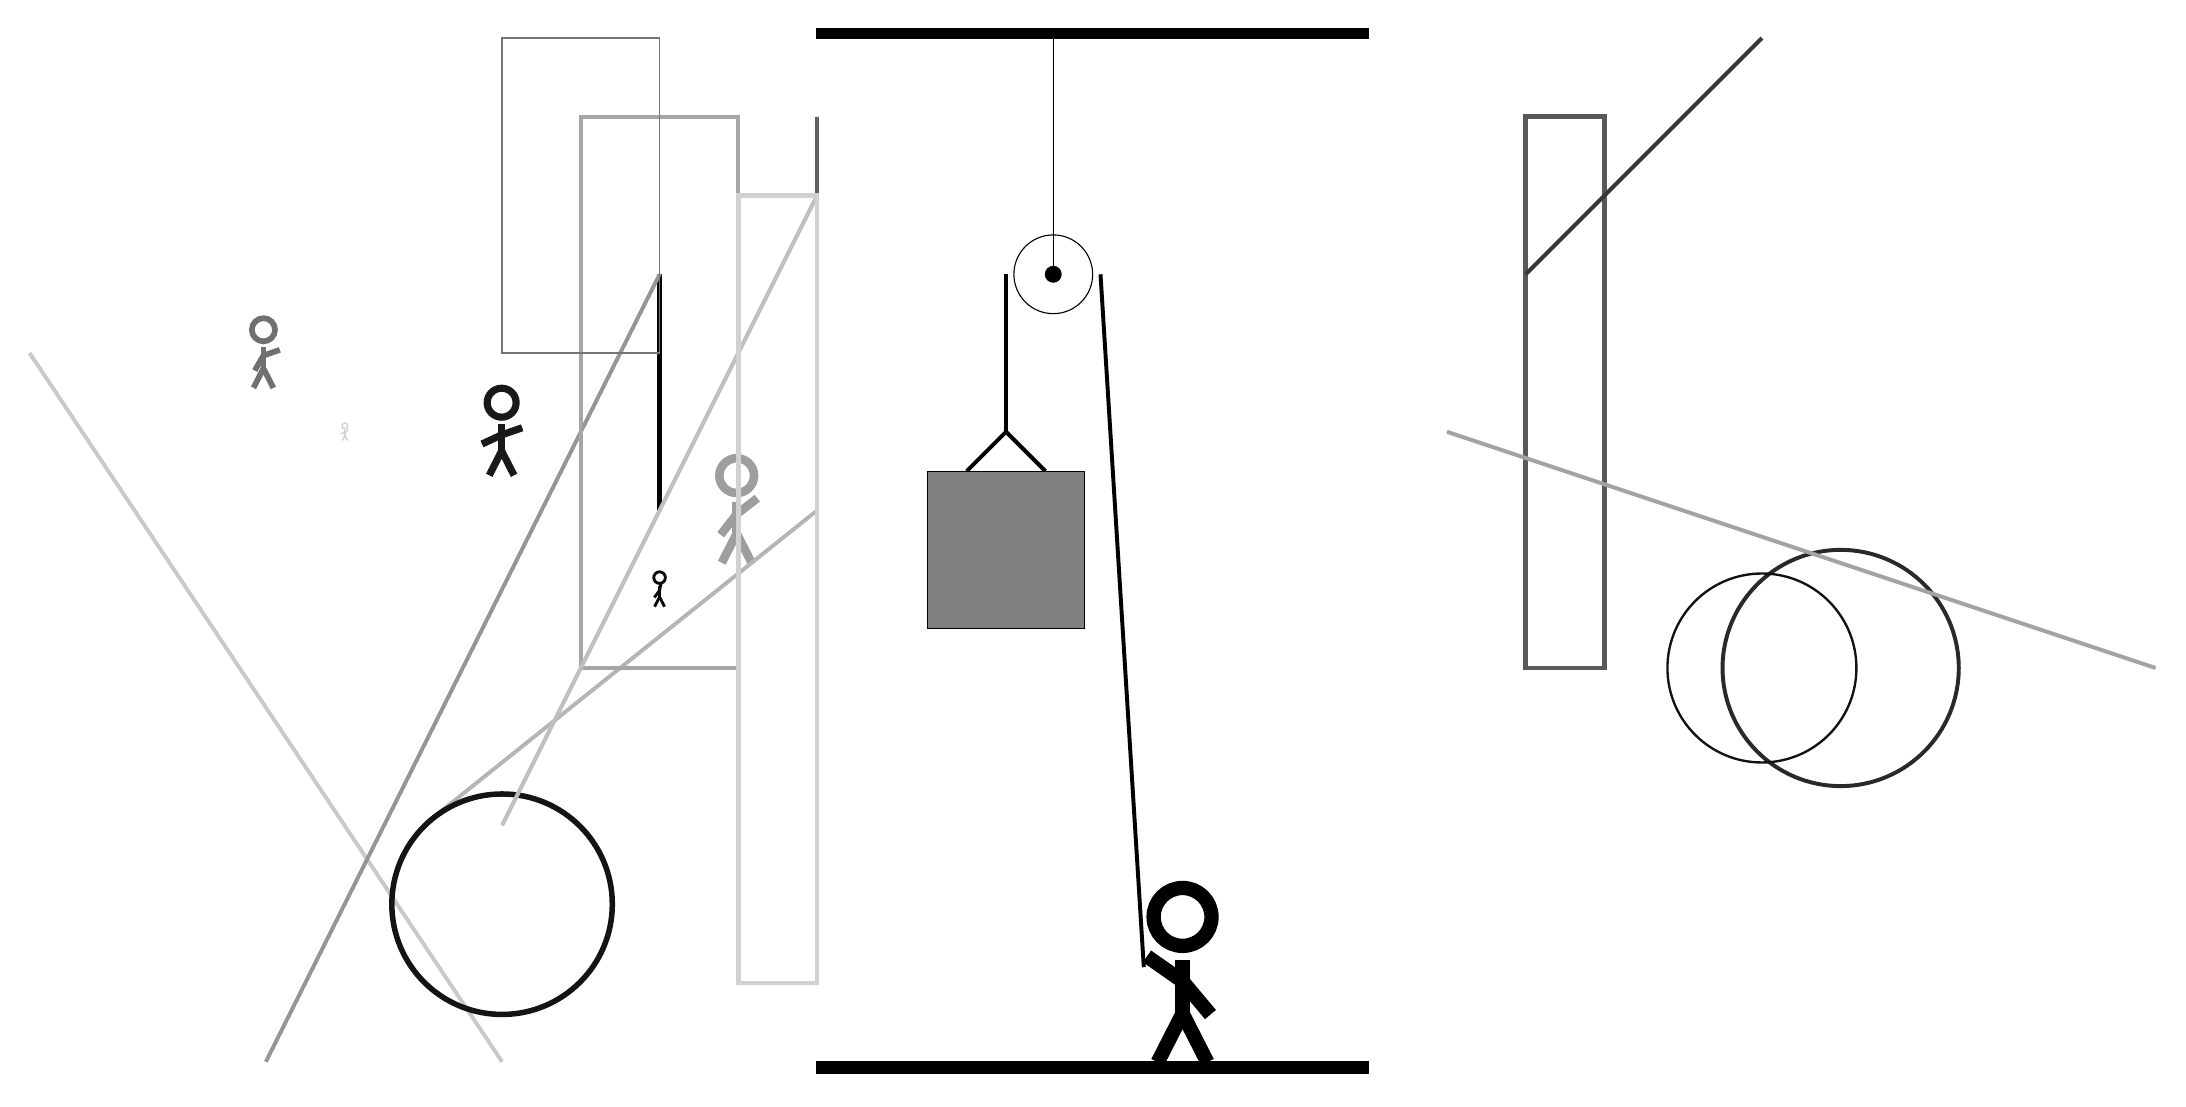
\begin{tikzpicture}
		%%%%% START %%%%%
		
		\draw[fill=black] (-2, 10) rectangle (5, 10.125);
		
		\draw (1, 7) circle (0.5);
		\draw[fill=black] (1, 7) circle (0.1);
		\draw (1, 10) -- (1, 7);
		
		\draw[line width=0.5mm] (-0.1, 4.5) -- (0.4, 5.0) -- (0.9, 4.5);
		\draw[fill=black!50] (-0.6, 4.5) rectangle (1.4, 2.5);
		
		\draw[line width=0.5mm] (0.4, 7) -- (0.4, 5.0);
		\centerarc[line width=0.5mm](1, 7)(0:180:0.6);
		\draw[line width=0.5mm](1.6, 7) -- (2.15, -1.8);
		
		\draw[line width=0.6mm, color=black!98] (-4, 7) rectangle (-4, 4);
		
		\draw[line width=0.5mm, color=black!21](-6, -3) -- (-12, 6);
		\draw [line width=0.5mm, color=black!84](11, 2) circle (1.5);
		\node[line width=0.5mm, color=black!97] at (-4, 3) {\Strichmaxerl[2][53][78]};
		\draw[line width=0.6mm, color=black!65] (7, 9) rectangle (8, 2);
		\node[line width=0.3mm, color=black!38] at (-3, 4) {\Strichmaxerl[6][52][38]};
		\draw[line width=0.5mm, color=black!41](-4, 7) -- (-9, -3);
		\draw[line width=0.5mm, color=black!29](-7, 0) -- (-2, 4);
		\draw [line width=0.3mm, color=black!93](10, 2) circle (1.2);
		\draw[line width=0.5mm, color=black!35] (-3, 2) rectangle (-5, 9);
		\draw[line width=0.2mm, color=black!54] (-4, 6) rectangle (-6, 10);
		\node[line width=0.2mm, color=black!90] at (-6, 5) {\Strichmaxerl[5][25][19]};
		\draw [line width=0.7mm, color=black!92](-6, -1) circle (1.4);
		
		\node[line width=0.3mm, color=black!56] at (-9, 6) {\Strichmaxerl[4][60][19]};
		\draw[line width=0.4mm, color=black!62] (-2, 5) rectangle (-2, 9);
		\draw[line width=0.5mm, color=black!25](-2, 8) -- (-6, 0);
		
		\draw[line width=0.5mm, color=black!36](6, 5) -- (15, 2);
		
		\draw[line width=0.5mm, color=black!78](10, 10) -- (7, 7);
		\draw[line width=0.6mm, color=black!18] (-2, 8) rectangle (-3, -2);
		\node[line width=0.7mm, color=black!18] at (-8, 5) {\Strichmaxerl[1][19][37]};
		
		\node at (2.6, -1.9) {\Strichmaxerl[10][-35][-50]};
		
		\draw[fill=black] (-2, -3) rectangle (5, -3.15);
		
		%%%%% END %%%%%
	\end{tikzpicture}
\end{document}